%%% File encoding: UTF-8
%%% äöüÄÖÜß  <-- keine deutschen Umlaute hier? UTF-faehigen Editor verwenden!

\documentclass[master,english]{hgbthesis}
% Zulässige Class Options:
%   Typ der Arbeit: diplom, master (default), bachelor, praktikum
%   Hauptsprache: german (default), english
%%%----------------------------------------------------------

\RequirePackage[utf8]{inputenc}		% Bei der Verw. von lualatex oder xelatex entfernen!

\graphicspath{{images/}}    % Abbildungsverzeichnis
\logofile{logo}				% Name des Logo-PDFs in images/ (\logofile{}, wenn kein Logo gewünscht)
\bibliography{literatur}  	% Name der Biblatex-Literaturdatei (.bib)

%%%----------------------------------------------------------
% Angaben für die Titelei (Titelseite, Erklärung etc.)
%%%----------------------------------------------------------

%%% Einträge für ALLE Arbeiten: -----------------------------
\title{Event-based build pipeline for static content management}
\author{Sascha Zarhuber}
\studiengang{Interactive Media}
\studienort{Hagenberg}
\abgabedatum{2017}{06}{11}	% {YYYY}{MM}{DD}

%%% Zusätzlich für eine Bachelorarbeit: ---------------------
\nummer{1510629021-A}   % Stud-ID, z.B. 1310238045-A
% (A = 1. Bachelorarbeit)
\semester{Sommersemester 2016}
\gegenstand{Einführung in die Tiefere Problematik 1}
\betreuer{FH-Prof. DI Rimbert Rudisch-Sommer} % oder \betreuerin{..}

%%% Restriktive Lizenformel anstatt CC (nur für Typ master) -
\strictlicense

%%%----------------------------------------------------------
\begin{document}
%%%----------------------------------------------------------

%%%----------------------------------------------------------
\frontmatter                    % Titelei (röm. Seitenzahlen)
%%%----------------------------------------------------------

\maketitle
\tableofcontents

\chapter{Vorwort} 	% engl. Preface


Dies ist \textbf{Version \hgbthesisDate} der \latex-Dokumentenvorlage für 
verschiedene Abschlussarbeiten an der Fakultät für Informatik, Kommunikation
und Medien der FH Oberösterreich in Hagenberg, die mittlerweile auch 
an anderen Hochschulen im In- und Ausland gerne verwendet wird.

Das Dokument entstand ursprünglich auf Anfragen von Studierenden,
nachdem im Studienjahr 2000/01 erstmals ein offizieller
\latex-Grundkurs im Studiengang Medientechnik und -design an der
FH Hagenberg angeboten wurde. Eigentlich war die Idee, die bereits
bestehende \emph{Word}-Vorlage für Diplomarbeiten "`einfach"' in
\latex\ zu übersetzen und dazu eventuell einige spezielle
Ergänzungen einzubauen. Das erwies sich rasch als wenig
zielführend, da \latex, \va was den Umgang mit Literatur und
Grafiken anbelangt, doch eine wesentlich andere Arbeitsweise
verlangt. Das Ergebnis ist -- von Grund auf neu geschrieben und
wesentlich umfangreicher als das vorherige Dokument --
letztendlich eine Anleitung für das Schreiben mit \latex, ergänzt
mit einigen speziellen (mittlerweile entfernten) Hinweisen für \emph{Word}-Benutzer.
Technische Details zur aktuellen Version finden sich in Anhang \ref{ch:TechnischeInfos}.

Während dieses Dokument anfangs ausschließlich für die Erstellung
von Diplomarbeiten gedacht war, sind nunmehr auch  
\emph{Masterarbeiten}, \emph{Bachelor\-arbeiten} und \emph{Praktikumsberichte} 
abgedeckt, wobei die Unterschiede bewusst gering gehalten wurden.

Bei der Zusammenstellung dieser Vorlage wurde versucht, mit der
Basisfunktionalität von \latex das Auslangen zu finden und -- soweit möglich --
auf zusätzliche Pakete zu verzichten. Das ist nur zum Teil gelungen;
tat\-säch\-lich ist eine Reihe von ergänzenden "`Paketen"' notwendig, wobei jedoch
nur auf gängige Erweiterungen zurückgegriffen wurde.
Selbstverständlich gibt es darüber hinaus eine Vielzahl weiterer Pakete,
die für weitere Verbesserungen und Finessen nützlich sein können. Damit kann
sich aber jeder selbst beschäftigen, sobald das notwendige Selbstvertrauen und
genügend Zeit zum Experimentieren vorhanden sind.
Eine Vielzahl von Details und Tricks sind zwar in diesem Dokument nicht explizit
angeführt, können aber im zugehörigen Quelltext jederzeit ausgeforscht
werden.

Zahlreiche KollegInnen haben durch sorgfältiges Korrekturlesen und
konstruktive Verbesserungsvorschläge wertvolle Unterstützung
geliefert. Speziell bedanken möchte ich mich bei Heinz Dobler für
die konsequente Verbesserung meines "`Computer Slangs"', bei
Elisabeth Mitterbauer für das bewährte orthographische Auge und
bei Wolfgang Hochleitner für die Tests unter Mac~OS.

Die Verwendung dieser Vorlage ist jedermann freigestellt und an
keinerlei Erwähnung gebunden. Allerdings -- wer sie als Grundlage
seiner eigenen Arbeit verwenden möchte, sollte nicht einfach
("`ung'schaut"') darauf los werken, sondern zumindest die
wichtigsten Teile des Dokuments \emph{lesen} und nach Möglichkeit
auch beherzigen. Die Erfahrung zeigt, dass dies die Qualität der
Ergebnisse deutlich zu steigern vermag.

Der Quelltext zu diesem Dokument sowie das zugehörige
\latex-Paket sind in der jeweils aktuellen Version online
verfügbar unter
%
\begin{itemize}
\item[]\url{https://sourceforge.net/projects/hgbthesis/}.
\end{itemize}
%
Trotz großer Mühe enthält dieses Dokument zweifellos Fehler und Unzulänglichkeiten
-- Kommentare, Verbesserungsvorschläge und passende Ergänzungen
sind daher stets willkommen, am einfachsten per E-Mail direkt an mich:
\begin{itemize}
\item[]%

Dr.\ Wilhelm Burger, Department für Digitale Medien,\newline
Fachhochschule Oberösterreich, Campus Hagenberg (Österreich)\newline
\nolinkurl{wilhelm.burger@fh-hagenberg.at}
\end{itemize}

\noindent
Übrigens, hier im Vorwort (das bei Diplom- und Masterarbeiten üblich, bei Bachelorarbeiten 
aber entbehrlich ist) kann kurz auf die Entstehung des Dokuments eingegangen werden.
Hier ist auch der Platz für allfällige Danksagungen (\zB an den Betreuer, 
den Begutachter, die Familie, den Hund, \ldots), Widmungen und philosophische 
Anmerkungen. Das sollte allerdings auch nicht übertrieben werden und sich auf 
einen Umfang von maximal zwei Seiten beschränken.




 % Optional. Ggf. weglassen
\chapter{Kurzfassung}

\begin{german}
Während moderne Content Management Systeme ein gut entwickeltes Umfeld für Online-Inhaltsverwaltung und -erstellung bereitstellen, sind sie doch auf eine Anzahl externer Services angewiesen. Dazu zählen vordergründig Datenbanksysteme, aber auch verschiedene Login-Mechanismen, um Zugang zu einem gesperrten Editierbereich freizugeben. Durch die Abhängigkeit von derartigen Services entsteht bei zunehmender Größe des jeweiligen Projekts ein Anstieg des Aufwands für die Verwaltung dieser Erweiterungen.

Static Site Generatoren andererseits benötigen keine externen Erweiterungen, da ihre einzige Aufgabe darin besteht, die Website-Quellcodes in eine für Webbrowser lesbare Version zu konvertieren. Allerdings haben diese Static Site Generatoren einen erheblichen Nachteil; da sie nicht zwischen bereits vorhandenen und neuen Inhalten unterscheiden können, ist jedesmal ein vollständiger Neubau der Website-Quellen notwendig.

Diese Masterarbeit soll daher einen Lösungsweg für dieses Problem aufzeigen. Durch einen selektiven Algorithmus sollen am Ende nur die wirklich notwendigen Inhalte gebaut werden und in eine vorhandene Dateistruktur eingebunden werden. Zusammen mit einer REST API soll zusätzlich eine benutzerfreundliche Interaktion und verbesserte Arbeitsteilung möglich sein.
\end{german}

\chapter{Abstract}

Whereas modern content management systems provide a solid environment for dynamic content creating and editing, their dependency on external services like database services or authentication providers often complicate their abilities to scale. Additional duties for keeping them responsive in larger ecosystems are therefore often responsible for slowing down the overall workflow of a developer.

Static site generators on the other hand offer an easy solution for steadily growing websites. Their only task is to create a full-featured file structure, which contains browser-readable HTML files that do not require any on-the-fly rendering upon request. However, static site generators contain a significant drawback, as the rendering mechanism normally cannot distinguish between already present files and new content. In fact, the build time increases every time a new file is added to the source directory.

This Master's thesis therefore tries to compensate the full extent of a complete rebuild every single build cycle by providing a caching mechanism based on a selective approach, together with a remotely working REST API as wrapping interface for user-friendly interaction and improved division of work.


%%%----------------------------------------------------------
\mainmatter          % Hauptteil (ab hier arab. Seitenzahlen)
%%%----------------------------------------------------------

%% Here comes the introduction
\chapter{Introduction}
\label{cha:introduction}
Back in the early 1990s, when the internet made its first steps towards a broader public use, a group of students at the University of Illinois created ``Mosaic'', the first publicly available Browser \cite[11]{dhillon2016}. At that time, websites consisted of just HTML and probably some images, whereas the release of ``Netscape Navigator'' led to the introduction of \emph{Brendan Eich}'s JavaScript engine. Additionally, Netscape also introduced a web server software called ``Netscape Enterprise Server'', thus making the Internet available for the first web developers \cite[12]{dhillon2016}.

Since then, a lot has changed; content management systems were published, the internet was turning to what was called ``Web 2.0'' and the common user was not just a content recipient anymore, but also a content creator without requiring deeper understanding of web technologies \cite[19]{dhillon2016}. This has affected not only private users, but also whole enterprise structures until today.

However, the most important part stayed the same; steadily providing content which is deliverable on request. To do so using content management systems requires not only a web server and the client's browser, but also a properly set up chain of interacting services for assembling HTML code on the fly. While this kind of architecture may surely be fitting smaller blogs very well, the necessary effort of managing constantly growing enterprise sites is likely to grow exponentially.

Therefore, systems which are not dependent on such a chain are constantly on the rise over the last yars. They especially make sense in environments, where content is constantly added, but hardly ever deleted or changed. Lastly, by constructing static websites in plain HTML and mostly avoiding any dynamic features, a trend reversal back to the internet origins is clearly noticeable in some fields of modern web development.

\section{Problem statement}
\label{sec:staticsitegenerators}
Static site generators are growing fast and are more and more used as a replacement for common content management systems. The main advantage is their independence of external services, like database systems, session caching services, etc. Also, they seldomly consist of complicated backend systems and are mostly created in pure HTML or simple markup languages like Markdown (see Sec. \ref{sec:buildpipelines-markdown}).

One of the biggest drawbacks however is the fact, that static site generators have to preprocess every bit of information they contain. This is the complete opposite compared to other content management systems, which process information on request. This means, that user-readable content is fetched and rendered ``just in time'' it was requested from the client.

Therefore, depending on the setup, a dynamically growing amount of time needed for a build cycle might be the case. For being able to work against this fact, a working approach has to be found, which saves time by leaving out information, which has not changed since the previous build.

\section{Goals}
\label{sec:goals}
To find a suitable solution, a service which contains a build pipeline including a caching mechanism has to be implemented. The caching mechanism should thereby act as the core part, as it is responsible for fetching data between the current development state and a previous build cycle. Furthermore it should determine the build extent by selecting the respective files for rendering based on the fetched commit diff. The research question is therefore the following:

\begin{center}
  How to speed up static site generation by a selective approach?
\end{center}
The implemented solution covers the necessary steps for working with cacheable content in a way, that a remote-only building process is possible. Together with the precondition of having a GitHub account, any repository consisting of a Metalsmith project should be able to get rendered on this service's REST API.

By introducing this service early into a project workflow, the user should notice a significant improvement concerning the rendering time per build cycle. Furthermore, it should take a considerable amount of workload out the developers hands.

\section{Structure}
\label{sec:structure}
To express the considerations which led to the finished solution, the following pages are structured into several chapters.

\begin{description}
  \item[Chapter 2] -- Shows the current state of the art, culminating in the presentation of three selected static site generators: \emph{Jekyll}, \emph{Hexo}, \emph{Metalsmith}, as well as a comparison between them.
  \item[Chapter 3] -- Explains the most important terms concerning the operation of static site generators (including code samples); \emph{build pipelines}, \emph{frontmatter}, \emph{markdown}, \emph{templates} and \emph{diff}.
  \item[Chapter 4] -- Gives an understanding of the initial theoretical approach behind this project. Challenges and solution strategies are examined prior to general considerations towards the implementation are being unveiled.
  \item[Chapter 5] -- Describes the full extent of the implementation including the whole REST framework, which was built around the build pipeline. Different graphics are showing examples of how various parts were realized.
  \item[Chapter 6] -- Evaluates the project using different testing approaches. The REST API was put under high load testing, whereas the build pipeline and the caching mechanism were compared using the timespan needed for an operation. Furthermore, an outlook shows possible future improvements.
  \item[Chapter 7] -- Shows the conclusion of this project work and unveils difficulties, as well as enhancement strategies for productive use.
\end{description}

% Transforming Web 1.0 to Web 2.0 - common user is not only content recipient anymore, also content creator
%% in the beginning, creating content on the internet was too difficult for the average Joe.

% Web 2.0 standards-based web, one way to measure is content creation
%% Blogs, social media, videos

% Blogging emerged as a solution to one of the biggest problems; not having enough people to create content

% Not just blogging software, also computer languages evolved

% Blogging will never die out, simply will take over a new form

\chapter{State of the art}
\label{cha:state-of-the-art}

%% W3Tech chart of server-side language share
\begin{figure}
    \centering
    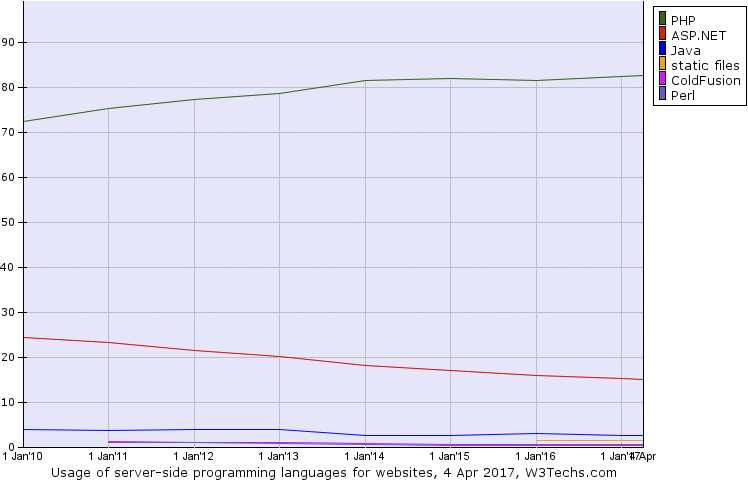
\includegraphics[width=0.9\textwidth]{server-side-languages.png}
    \caption{A graphic showing the global share of \emph{server-side programming languages} from January 2010 to April 2017. \emph{PHP} remains the dominant language with a share growing from 72.5\% to 82.6\%.\\
    Source: \url{https://w3techs.com/technologies/history_overview/programming_language/ms/y}}
    \label{fig:server-side-languages}
\end{figure}
%

\paragraph{} % History of Content Management Systems.
The roots of the most well-known modern Content Management Systems (\emph{CMS}) date back to the early 2000s, when PHP was (and \emph{still is}) the dominant factor in terms of server-side programming languages (see Fig. \ref{fig:server-side-languages}). %% Please check, if reference is accurate enough

While the \emph{typical} CMS was starting out as mostly just a ``dynamic online tool'', it also shows that with seamlessly integrating new features gained through the development of its underlying programming languages, as well as steadily adding new functionalities (mostly requested by the community), a transition towards a fully-manageable and customizeable, semi-automatic web application was possible \cite[17]{dhillon2016}.

The advantages are clear; A web designer or content editor does not automatically have to be a web developer, who needs profound knowledge about software or server architecture. Instead, most of the time it is enough to know how to operate an FTP-client and to know the credentials of the built-in database service, submitted by the web hosting provider upon registration.\\
As a summary, it can be said: \emph{Less people for less responsibilities} -- The web application does the rest.

However, this progression also caused a few drawbacks, especially when it comes down to comparing the amount of workload needed before actually being able to create content for the World Wide Web. Due to the fact, that most CMSs evolved to their own sort of powerful admin panels, developers who are not keen about keeping their site updated, risk its defacing or other embarrassing attacks through unmanaged security holes in the code \cite[23]{dhillon2016}.\\
So, how is it possible to bridge the gap between a fairly secure system and creating content whenever it is desired?

\paragraph{} % Creating content using static HTML.
\label{par:creatingcontent}
In 2008, \emph{Tom Preston-Werner} created \emph{Jekyll} out of his frustration of having the need of ``styling a zillion template pages'' and ``moderating comments all day long'' before even being ready to create content on his blogging engine \cite[]{PrestonWerner2008jekyll}. Furthermore he mentioned, that one of the other main reasons were the lack of possibility for publishing his posts on his own server, when subscribing to a fully-managed online hosting service like \texttt{wordpress.com}\footnote{\url{https://en.wordpress.com} -- A hosted version of Wordpress.}. Services like this offer only limited customization options, where there likely is no access to online storage and database without using the built-in admin panel. Even then, access might be very restricted.

The intended core functionality of Jekyll narrows down its mode of operation to handle three main components found in most static site generators today \cite[24]{dhillon2016}:

\begin{description}
  \item [Core language] -- The language a static generator is written in, for example JavaScript or Ruby.
  \item [Templates] -- The templating language to be used through the blog and posts.
  \item [Plug-ins] -- All static site generators allow for additional functionality through some
sort of a plug-in system.
\end{description}

In contrast to common dynamic CMSs, a static site generator outputs plain static HTML. It does it in a way, that a certain \emph{distribution} folder holds the complete web root, without the need of binding it to external services like databases or session management tools. Occasionally, different plug-ins also allow the generation of client-side \emph{JavaScript} or \emph{Cascading Style Sheet} files through their respective pre-processing tools.

\section{Jekyll}
\label{sec:jekyll}

As already explained, Jekyll was created out of the need for avoiding to service the blogging engine before writing and publishing content. Since it is deeply integrated into \emph{GitHub}, it is considered as the probably most-popular static site generator.

\subsection{History}
\label{sec:jekyll-history}
\emph{Tom Preston-Werner}, co-founder of GitHub\footnote{\url{https://github.com} -- GitHub Inc.}, announced it in October 2008 in one of his blog posts \cite{PrestonWerner2008jekyll}. Already in December 2008, it was introduced as build engine for the then newly featured GitHub Pages service, allowing owners of repositories to publish a static website by just pushing to a certain \emph{master} or \emph{gh-pages} branch \cite{PrestonWerner2008githubpages}, which is still available for free to this day.

All of this happened just 6 (respectively 8) months after GitHub was launched \cite{PrestonWerner2008githublaunch} and is now even being used by technology-leading companies to showcase their Open-Source efforts\footnote{\url{https://github.com/showcases/github-pages-examples} -- GitHub Pages examples.}.

\subsection{Technology}
\label{sec:jekyll-technology}
Jekyll was entirely written in \emph{Ruby}, as Tom Preston-Werner rather saw himself as a software developer in the first place, than as a content author \cite{PrestonWerner2008jekyll}. Until now, the repository for Jekyll still consists mainly of Ruby code at a share of roughly 77.5\%.

\subsubsection{Advantages}
One of the main advantages is the modular structure of its code base. By inheriting different Ruby classes, it is quite easy to extend and add features to fit the developer's needs. Due to its wide-spread usage initiated through the GitHub universe, Jekyll also has an accordingly huge user base and is therefore well documented \cite[26]{dhillon2016}.

Furthermore, its website\footnote{\url{http://jekyllrb.com} -- Jekyll website.}, which mainly acts as starting basis for documentation, is not only available as open-sourced git repository, it is also built using \texttt{Jekyll} to prove its universality.

Starting from scratch, the command \texttt{jekyll new my\_project} installs a blog environment for starters in the \texttt{./my\_project} folder. The basic install consists of an elementar blog post structure, \emph{Sass} source files, and a few template files written for Shopify's \emph{Liquid}\footnote{\url{https://help.shopify.com/themes/liquid} -- Shopify's Liquid template engine.} engine.\\
Using this starting environment, the unexperienced developer quickly gets a sufficient overview of what is generally possible using Jekyll, whereas the content author is able to fully concentrate himself on writing content, as the used \emph{Markdown} markup language requires little to no prior syntax knowledge. Furthermore, Jekyll already ships with a built-in webserver for quickly reviewing the rendered static output.

\subsubsection{Disadvantages}
As powerful as Ruby might be designed, many unskilled developers are facing difficulties right from the beginning, as most of them experience a steep learning curve. Nearly every single bit of customizing Jekyll requires Ruby knowledge, especially if it is desired to move along the ``predefined'' way and not including third-party extensions like \emph{Node.js} tools or else.

Additionally, its template language, Liquid, offers customization on a very high level, so it might happen to confuse business logic\footnote{How Jekyll processes data into programmatically readable structures.} with template logic\footnote{How Liquid transforms these structures into browser-readable HTML.}. To make things worse, different template constructions might also evolve over time and therefore causing a parallel coding universe when trying to surpass difficulties in the business logic.

%% bring some difficulties concerning ruby versions
%% ruby gems

\section{Hexo}
\label{sec:hexo}

\texttt{Hexo} understands itself as counterpart to \texttt{Jekyll}, mostly by covering the same ideas of static site generation, but building up completely on \texttt{Node.js}. It even offers a migration service for \texttt{Octopress}- and \texttt{Jekyll}-users who are willing to switch.

\subsection{History}
\label{sec:hexo-history}
\texttt{v1.0.0} was originally released in March 2013\footnote{\url{https://github.com/hexojs/hexo/releases/tag/1.0.0} -- Hexo v1.0.0 release page on \texttt{GitHub}.}, although development on \texttt{GitHub} dates back to September 2012 as the first commit was published using the message \emph{``init''}.

\emph{Tommy Chen}, its creator, first used \texttt{Octopress}\footnote{\url{http://octopress.org} -- Octopress website.} but quickly became dissatisfied with its performance, as the rendering of 54 blog posts already took more than a minute of compile time \cite{Chen2012hexodebut}. Since he assumed \texttt{Ruby} might be the cause for the lack of performance of his primarily used blogging framework, and further development on this case was not likely to happen any time soon, he decided to look for something which got his attention shortly before: \texttt{Node.js}.

However, \texttt{Node.js} was not really a big player back at that time, so the offer of blogging frameworks written in \texttt{JavaScript} was very dense and not really fitting the needs of \emph{Tommy Chen}. In his announcement article for \texttt{Hexo} \cite{Chen2012hexodebut}, he references a blog post of \emph{Boris Mann}, also an \texttt{Octopress} user at that time, listing a few \texttt{Node.js}-based blogging frameworks, which were already around in June 2012\footnote{\url{http://blog.bmannconsulting.com/node-static-site-generators} -- Blog article of \emph{Boris Mann} about \texttt{Node.js}-based blogging frameworks.}. Interestingly, only two of all the mentioned ones, \texttt{Wintersmith} and \texttt{DocPad} are still actively maintained today.

\subsection{Technology}
\label{sec:hexo-technology}
As already stated above, \texttt{Hexo} primarily consists of \texttt{JavaScript}, thus making it easier to start for developers with a front-end web development background. In fact, its \texttt{GitHub} repository shows \texttt{JavaScript} holding a share of 100\% on the source code\footnote{\url{https://github.com/hexojs/hexo} -- Hexo repository on \texttt{GitHub}.}.

\subsubsection{Advantages}
Right from the start, \texttt{Hexo} presents itself using its feature-rich command-line interface (\emph{CLI}), similar to \texttt{Jekyll}. Once it is installed, \texttt{hexo init my\_project} scaffolds a new starter template into the \texttt{./my\_project} folder.\\
As \emph{Tommy Chen} himself wanted an easy-to-use replacement for \texttt{Octopress}, \texttt{Jekyll} and \texttt{Hexo} share a lot of common features; their content files use both \texttt{YAML} frontmatter and \texttt{Markdown} by default, even the main configuration file uses a very similar structure in both frameworks. This should make it extremely easy switching from \texttt{Jekyll} to \texttt{Hexo}.

First and foremost, programming-unaware content authors might especially like its CLI, as it also offers to create files based on the \texttt{hexo new} command. Depending on other submitted command-line arguments, \texttt{Hexo} may automatically put the new post in the according sub-folder, whether it is a \emph{draft, page} or \emph{post}. Publishing a draft is as easy as \texttt{hexo publish}.\\
When creating content, \texttt{Hexo} also contains a feature-rich, \texttt{Octopress}-inspired custom tag selection for including content from \emph{YouTube, Vimeo} or \emph{GitHub Gists}.

Additionally, its plugin collection is also constantly growing and mostly community supported. A special naming convention using \texttt{hexo-} as prefix helps by determining which plugins to auto-load out of the \texttt{node\_modules} folder. Using this way, \texttt{Ruby's} \emph{convention over configuration} mantra is ported to \texttt{JavaScript} as well and supports especially beginners by not having to define the usage of a certain plugin.

\subsubsection{Disadvantages}
\texttt{Hexo} might look like as an ideal replacement for \texttt{Jekyll}, but since both share so much similarities, they also share some disadvantages. Whereas \texttt{Jekyll} ships with \emph{Liquid} and \emph{Sass} as standard, \texttt{Hexo} does with \emph{EJS} and \emph{Stylus}.\\
Although clearly stated, that both of these plugins might be easily uninstalled later on\footnote{\url{https://hexo.io/docs/setup.html\#package-json} -- Hexo's setup documentation.}, the whole setup pre-installation seems as opinionated as \texttt{Jekyll's}.

In addition to the already mentioned plugin system, a missing configuration option might as well turn out to be misleading in terms of customization options, especially when being dependent on the CLI. If customization is necessary, the developer often is forced to switch to the \texttt{JavaScript} API\footnote{\url{https://hexo.io/api/} -- Hexo's JavaScript API documentation.} or add a plugin to the project to make the build pipeline fit the customization's needs.

When it comes to caching, \texttt{Hexo} uses a homebrew version of \emph{JSON memory caching} called \texttt{Warehouse}, also created by \emph{Tommy Chen}\footnote{\url{https://github.com/tommy351/warehouse} -- Warehouse repository on \texttt{GitHub}.}, initially mentioned in the release notes of \texttt{3.2.0-beta.2} \cite{Chen2015hexorelease}. Using this plugin, a mode called ``Hot processing'' should enable faster re-builds. The main drawback here might be the caching speed, which is on the one hand filling up the memory when working on bigger projects, whereas the persisting of the database is fully dependent on file input/output write speeds of the underlying hard disk.\\
Furthermore, a constantly growing database file is hardly transferrable when trying to implement a decentralized building system out of \texttt{Hexo}.

\section{Metalsmith}
\label{sec:metalsmith}

Compared to the already described static site generators, \texttt{Metalsmith} is to be considered the youngest project.
It might also be the most radical project, as it was designed to consist of \textbf{nothing but plugins} \cite[31]{dhillon2016}. Therefore, in terms of still being a static site generator, it tries hard to push the limits much further than previously mentioned \texttt{Jekyll} and \texttt{Hexo}.

\subsection{History}
\label{sec:metalsmith-history}
Initially developed by \emph{Segment}\footnote{\url{https://segment.com} -- Segment's website.} for their internal needs, such as \emph{documentation, help} and \emph{blog pages} \cite{Metalsmith2015buildingblocks}, \texttt{Metalsmith} was finally open-sourced and made publicly available around February 2015 -- its commit history on \texttt{GitHub} dates back to February 4\textsuperscript{th}, 2014.\\
Most of the commits at that time were published by \emph{Ian Storm Taylor}, co-founder of \emph{Segment}, although his contribution to the project ends after releasing \texttt{v2.1.0} on September 24\textsuperscript{th}, 2015\footnote{\url{https://github.com/segmentio/metalsmith/commits/master?author=ianstormtaylor} -- Contributions of \emph{Ian Storm Taylor} to the Metalsmith repository on \texttt{GitHub}.} at the moment.

Like \texttt{Hexo}, \texttt{Metalsmith's} repository completely consists of \texttt{JavaScript} code, as its developers also were unsatisfied with the then existing static site generators. According to \emph{Chris Sperandio}, the \texttt{Metalsmith} developers desired pure flexibility for their ``wide array of use cases'', while other frameworks all asked for a certain structure on the content \cite{Metalsmith2015buildingblocks}.

\subsection{Technology}
\label{sec:metalsmith-technology}
Since \texttt{Metalsmith} consists of only plugins, specifically written for this very framework, there is no real standard setup provided. Although there are a few tutorials and best practices listed in its \texttt{GitHub} repository\footnote{\url{https://github.com/segmentio/metalsmith\#the-secret} -- Possibilities for using Metalsmith.}, as well as in a repository called ``\emph{awesome-metalsmith}''\footnote{\url{https://github.com/metalsmith/awesome-metalsmith} -- ``Awesome'' Metalsmith resources list.}, the initial dive-in might scare a few people away, since \texttt{Metalsmith} might not be as well documented as the previously mentioned frameworks. Moreover, most developers seem to experience a very steep learning curve at first, given the amount of customization options and the requirements for understanding the blog engine~infrastructure \cite[31]{dhillon2016}.

\subsubsection{Advantages}
Every developer is able to shape \texttt{Metalsmith} exactly to his/her needs, once he knows about the basic usage. It ships with a CLI, as well as a \texttt{JavaScript} API, where the ``real hacking'' is possible.\\
The CLI gets easily configured via a \texttt{metalsmith.json} file, stored in the project directory. It consists mainly of general project configurations, placed in the object's root, as well as an array of used plugins, respectively combined with their configuration.

It neither contains a pre-installed template engine, nor any other pre-processing tools, like \texttt{Sass} or \texttt{Less}. However, the available plugins support most of them to a satisfying extent. As an example, the \texttt{metalsmith-layouts} plugin is a wrapper for \texttt{consolidate.js}, which per se acts as a wrapper for the most common template engines\footnote{\url{https://github.com/tj/consolidate.js\#supported-template-engines} -- Consolidate.js-supported template engines on \texttt{GitHub}.}. Therefore, the developer is able to select the tools based on his/her preferences and may initialize a project from scratch, without needing to clean up any pre-installed demonstration files first.

Using the built-in \texttt{JavaScript} API, it is also possible to invoke the needed modules programmatically, which is one of the core topics of this Thesis.

\subsubsection{Disadvantages}
So much freedom in designing a project may also cause some dangers. In this case, one of the most crucial things is the arrangement of plugins in the configuration. Since \texttt{Metalsmith} acts as a streaming build system, every transformation of the content must happen at its time to not interfere with any upcoming plugins. This is especially important when a plugin might alter the underlying code in a way, that a following plugin becomes useless, as it might not be able to succeed in its predefined task. \emph{Andy Jiang} gives a good example about a sample structuring of \texttt{Metalsmith} plugins on the \emph{Segment} blog \cite{Metalsmith2015technicaldocumentation}.

As an example, the following code snippet shows one bold example of misconfiguration (See line no. 16):

%% Update line no. above, if code changes
\lstinputlisting[language=JavaScript]{chapters/02-state-of-the-art/_support/metalsmith.js}

%% Screenshot of npms.io for search query metalsmith static assets
\begin{figure}[b] % h-ere, t-op, b-ottom, p-age
    \centering
    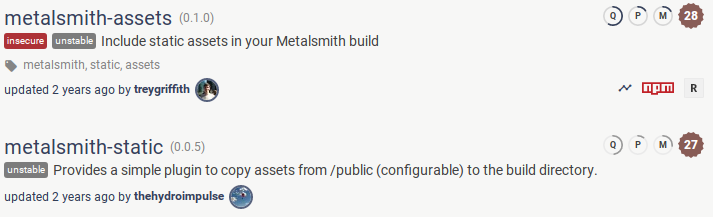
\includegraphics[width=0.9\textwidth]{metalsmith-static-plugins.png}
    \caption{A screenshot showing some of the results for the search query ``\emph{metalsmith static assets}'' on \url{https://npms.io}. Both of the shown entries describe an identical mode of operation within the \texttt{Metalsmith} build pipeline.\\
    Also notice the very unstable \texttt{semver} versions: \textbf{0.1.0} and \textbf{0.0.5}.}
    \label{fig:metalsmith-plugins}
\end{figure}
%

Moreover, the available plugins may seem as not as popular as the plugins from \texttt{Hexo}, given the average amount of stars received on \texttt{GitHub}. This might be due to the often missing maintainance, or simply because of the fact, that there seem to be multiple plugins for one single task (See Fig. \ref{fig:metalsmith-plugins}).

\section{Comparison}
\label{sec:comparison}

To conclude the summaries of different static site generators, a short overview using a table is given below (see Table \ref{table:comparison}). The comparison is built up on advantages and disadvantages, as well as the most important features they consist of. Therefore overall popularity and customizability play an as important role, as the language they are written in. However, Metalsmith stands a little bit out, as it does not provide a full-featured framework -- it merely serves as the basis for further plugin setup, whereas Jekyll and Hexo already contain some sort of standard setup.
The numbers of plugins in Table \ref{table:comparison} were taken from search queries on \url{https://npms.io} and \url{https://rubygems.org}.

\begin{table}
  \caption{A comparison of static site generators}
  \label{table:comparison}
  \centering
  \setlength{\tabcolsep}{5mm}
  \def\arraystretch{1.25}
  \begin{tabular}{|r||c|c|c|}
    \hline
    & \emph{Jekyll} & \emph{Hexo} & \emph{Metalsmith} \\
    \hline
    \hline
    Language & Ruby & JavaScript & JavaScript \\
    \hline
    Foundation & Oct. 2008 & Sept. 2012 & Feb. 2014 \\
    \hline
    Contributors & \textasciitilde 700 & \textasciitilde 100 & \textasciitilde 50 \\
    \hline
    Plugins & \textasciitilde 800 & \textasciitilde 600 & \textasciitilde 590 \\
    \hline
    Customizability & Mediocre & Low & High \\
    \hline
    Opinionatedness & High & High & Low \\
    \hline
    Standard templates & Liquid & Swig & \emph{none} \\
    \hline
  \end{tabular}

\end{table}



%%%----------------------------------------------------------
\appendix                                            % Anhang
%%%----------------------------------------------------------

%\chapter{Technische Informationen}
\label{ch:TechnischeInfos}

\newcommand*{\checkbox}{{\fboxsep 1pt%
\framebox[1.30\height]{\vphantom{M}\checkmark}}}

\section{Aktuelle Dateiversionen}

\begin{center}
\begin{tabular}{|l|l|}
\hline
Datum & Datei \\
\hline\hline
\hgbthesisDate & \texttt{hgbthesis.cls} \\
\hline
\hgbDate       & \texttt{hgb.sty} \\
\hline
\end{tabular}
\end{center}




\section{Details zur aktuellen Version}


Das ist eine völlig überarbeitete Version der DA/BA-Vorlage, die
\mbox{UTF-8} kodierten Dateien vorsieht und ausschließlich im PDF-Modus arbeitet.
Der "`klassische"' DVI-PS-PDF-Modus wird somit nicht mehr unterstützt! 

\subsection{Allgemeine technische Voraussetzungen}

Eine aktuelle \latex-Installation mit
\begin{itemize}
	
		\item Texteditor für \mbox{UTF-8} kodierte (Unicode) Dateien,
		\item \texttt{biber}-Programm (BibTeX-Ersatz, Version $\geq 1.5$),
		\item \texttt{biblatex}-Paket (Version $\geq 2.5$, 2013/01/10),
		\item Latin Modern Schriften (Paket \texttt{lmodern}).%
			\footnote{\url{http://www.ctan.org/pkg/lm}, \url{http://www.tug.dk/FontCatalogue/lmodern}}
\end{itemize}


\subsection{Verwendung unter Windows}

Eine typische Installation unter Windows sieht folgendermaßen aus
(s.\ auch Abschnitt \ref{sec:Windows}):
%
\begin{enumerate}
\item \textbf{MikTeX 2.9}%
	\footnote{\url{http://www.miktex.org/} -- \textbf{Achtung:} 
	Generell wird die \textbf{Komplett\-installation} von MikTeX ("`Complete MiKTeX"') empfohlen, 
	da diese bereits alle notwendigen Zusatzpakete und Schriftdateien enthält! 
	Bei der Installation ist darauf zu achten, 
	dass die automatische Installation erforderlicher Packages 
	durch "`\emph{Install missing packages on-the-fly: = Yes}"' ermöglicht wird (NICHT "`\emph{Ask me first}"')!
	Außerdem ist zu empfehlen, unmittelbar nach der Installation von MikTeX mit dem Programm
	\texttt{MikTeX} $\to$ \texttt{Maintenance} $\to$ \texttt{Update} und \texttt{Package Manager} 
	ein Update der installierten Pakete durchzuführen.}
	(zurzeit am einfachsten die 32-Bit Version, da nur diese das Programm \texttt{biber.exe} 
	bereits enthält),
\item \textbf{TeXnicCenter 2.0}%
	\footnote{\url{http://www.texniccenter.org/}}
	(Editor-Umgebung, unterstützt UTF-8),
\item \textbf{SumatraPDF}%
	\footnote{\url{http://blog.kowalczyk.info/software/sumatrapdf/}} 
	(PDF-Viewer),
\end{enumerate}
%
Ein passendes TeXnicCenter-Profil für MikTeX, Biber und Sumatra ist in diesem Paket enhalten
(Datei \verb!_tc_output_profile_sumatra_utf8.tco!). Dieses sollte man zuerst
über \texttt{Build} $\to$ \texttt{Define Output Profiles} in TeXnicCenter importieren.
\textbf{Achtung}: Alle neu angelegten \texttt{.tex}-Dateien sollten in UTF-8 Kodierung gespeichert werden!




\subsection{Verwendung unter Mac~OS}


Diese Version sollte insbesondere mit \emph{MacTeX} problemlos laufen (s.\ auch Abschnitt \ref{sec:MacOs}):
\begin{enumerate}
\item 
	\emph{MacTex} (2012 oder höher).
\item 
	Die Zeichenkodierung des Editors sollte auf UTF-8 eingestellt sein.
\item 
	Als Engine (vergleichbar mit den Ausgabeprofilen in TeXnicCenter) sollte \emph{LaTeXMk} verwendet werden. 
	Dieses Perl-Skript erkennt automatisch, wie viele Aufrufe von \emph{pdfLaTeX} und \emph{Biber} nötig sind. 
	Die Ausgabeprofile \emph{LaTeX} oder \emph{pdfLaTeX} hingegen müssen mehrmals aufgerufen werden, 
	zudem werden hierbei auch die Literaturdaten nicht verarbeitet. Dazu müsste extra die \emph{Biber}-Engine 
	aufgerufen werden, 	die jedoch noch nicht in allen Editoren vorhanden ist.
\end{enumerate}


\begin{comment}
\subsection{Vorteile}
\begin{itemize}
\item PDF wird direkt erzeugt ohne DVI und PS; damit ist angeblich auch die "`Feintypographie"' besser.
\item Die Verwendung von \texttt{SumatraPDF} erlaubt funktionierende Forward- und Inverse-Suche, womit erstmals ein effektiver PDF-Workflow möglich ist.
\item Preview der vollständigen Manuskripts (inklusive Grafiken) ist in PDF viel schneller
als in DVI (mit YAP und Ghostscript für die Grafiken).
\item Grafiken können auch als PDF, PNG oder JPEG direkt eingebunden werden. Bestehende EPS-Grafiken werden automatisch in PDF konvertiert. 
\item Bei eingebundenen Rasterbildern werden (im Unterschied zu \texttt{ps2pdf} in der Default-Einstellung) keine zusätzlichen JPEG-Artefakte erzeugt. 
(Anmerkung: im TC-Ausgabeprofil für \texttt{ps2pdf} ist dafür jetzt die
Option \verb!-dPDFSETTINGS=/prepress! eingestellt -- \verb!=/printer! ist nicht ausreichend!)
\item Die Erzeugung von aktiven Verweisen mit \texttt{hyperref} funktioniert problemlos, mit allen Vorteilen (einschließlich der Zeilenumbrüche in URLs).
\item PDF-Metadaten (zur verbesserten Suche) werden direkt aus den Dokumentendaten durch LaTeX generiert.
\end{itemize}

\subsection{Weitere Neuerungen}
%
\begin{sloppypar}
\begin{itemize}
\item Verwendung des \texttt{epstopdf}-Pakets, wodurch vorhandene EPS-Grafiken (mit denen \texttt{pdflatex} nicht umgehen kann) automatisch in PDF-Dateien konvertiert werden, unter der Annahme, dass \texttt{epstopdf.exe} vorhanden ist. Das ist bei Rasterbildern allerdings nicht zu enpfehlen, weil mit \texttt{epstopdf} die Kompressionsqualität nicht gesteuert erden kann. In diesem Fall ist es besser, die EPS-Dateien (\zB\ mit PhotoShop) direkt in PDFs zu konvertieren oder (noch besser) die Original JPEG- oder PNG-Dateien zu verwenden.
%
\item Unter \texttt{pdflatex} können nun (mit \verb!\includegraphics{}!) neben PDFs auch Bilder im JPEG- oder PNG-Format direkt eingebunden werden. Alle Datei-Extensions der Grafikdateien wurden im Quelltext entfernt.
%
\item 
Verwendung des \textbf{SumatraPDF}-Viewers anstelle von Adobe Acrobat, da Acrobat das Überschreiben der Ausgabedatei blockiert (unter Windows) und forward/inverse Suche schlecht \bzw\ gar nicht unterstützt.
Anweisungen zur Einstellung findet man unter \url{http://www.hehn.biz/Mar/How_to_Sumatra.pdf} -- diese sind auch im beiliegenden TC-Aus\-gabe\-profil implementiert.
%
\item Verwendung des \texttt{pdfsync}-Pakets zur Unterstützung der inversen Suche aus PDF-Dateien.
%
\item Verwendung des \texttt{hyperref}-Pakets zur Aktivierung von Links (Web, Inhaltsverzeichnis, Querverweise, Literatur etc.). Erzeugt auch eine Navigation-Pane.
%
\item PDF-Metadaten werden automatisch aus den Dokumentendaten generiert (durch \texttt{hyperref} möglich).
%
\item Verwendung des \texttt{breakurl}-Pakets, mit dem Zeilenumbrüche trotz \texttt{hy\-per\-ref} auch bei DVI-PS-PDF-Generierung durchgeführt werden. Dadurch sind jetzt auch URLs in Captions und Fußnoten problemlos möglich und auch \verb!\urldef{}! ist nicht mehr erforderlich (entspr.\ Textpassagen in \ref{sec:QuellenangabenInCaptions} entfernen!). 
%
\item Alle bestehenden EPS-Dateien mit Rasterbildern wurden auf Binärkodierung umgestellt, da dies mit der aktuellen MikTeX-Version keine Probleme mehr verursacht. Zusätzlich wurden PNG-Versionen für \texttt{pdflatex} angelegt, sodass keine automatische Umwandlung mit \texttt{epstopdf} erfolgt.
%
\item
Das lästige Problem des übermäßigen vertikalen Abstände in LaTeX-Aufzählungslisten wurde mit dem \texttt{enumitem}-Paket behoben. Alle \verb!\itemsep0pt! Anweisungen im Text wurden entfernt.
%
\item Einbindung des \texttt{cite}-Pakets mit \texttt{noadjust}-Option, womit kein zusätzliches Spacing erzeugt wird.
\end{itemize}
\end{sloppypar}
\end{comment}


\begin{comment}
\section{Einstellungen unter Windows} 
\label{sec:EinstellungAusgabeprofile}

Die folgenden Angaben beziehen sich auf eine bewährte Arbeitsumgebung unter Windows (XP, Win7) mit MikTeX, Sumatra-PDF und TeXnicCenter, mit folgenden Installationspfaden:
%
\begin{quote}
\verb!C:\Program Files (x86)\MiKTeX 2.9\! \\
\verb!C:\Program Files (x86)\SumatraPDF\! \\
\verb!C:\Program Files (x86)\TeXnicCenter\! 
\end{quote}
%
Unter Windows XP liegen die Programme in \verb!C:\Program Files\!.
Falls neuere Versionen dieser Komponenten installiert sind, müssen natürlich die nachfolgend angegebenen Pfade entsprechend modifiziert werden.

\begin{quote}
\textbf{Achtung:} Für MikTeX immer die \textbf{komplette Version} installieren! Das entsprechende Installationsverzeichnis hat aktuell einen Umfang von ca.\ 1.2 GB und enthält etwa 53.200 Dateien 
(typischerweise in \nolinkurl{C:\\Program Files (x86)\\MiKTeX...}).
\end{quote}
\end{comment}

\begin{comment}
\subsection{TeXnicCenter-Ausgabeprofile}
\label{sec:TeXnicCenterUndMikTeX}

TeXnicCenter definiert den Verarbeitungsablauf des LaTeX-Dokuments anhand von Ausgabeprofilen, wobei die oben genannten Komponenten als externe Programme mit entsprechenden Argumenten aufgerufen werden.
Die Einstellung der Ausgabeprofile erfolgt in TeXnicCenter über das Menü
\textsf{Ausgabe}$\rightarrow$\textsf{Ausgabeprofile definieren...} (Abb.\ \ref{fig:techniccenter-profile-latex}). 
Die Profile werden (abhängig von der installierten Software) üblicherweise beim ersten Start von TeXnicCenter durch den zugehörigen "`Wizard"' voreingestellt. 

\begin{figure}
\centering\small
\setlength{\tabcolsep}{0pt}%
\begin{tabular}{c@{~}c}
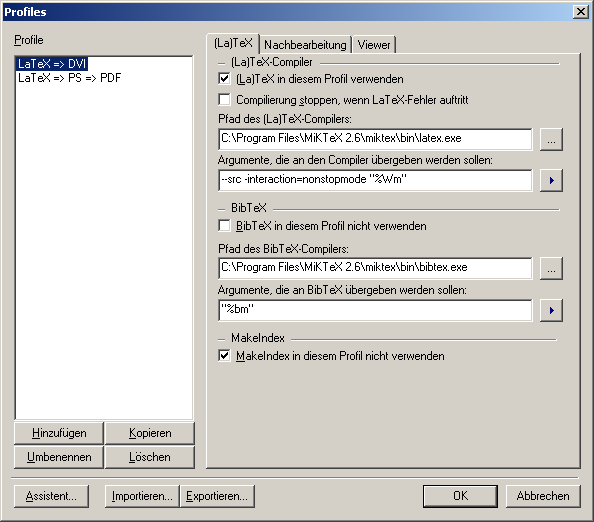
\includegraphics[width=0.49\textwidth]{techniccenter-profile-dvi-26} &
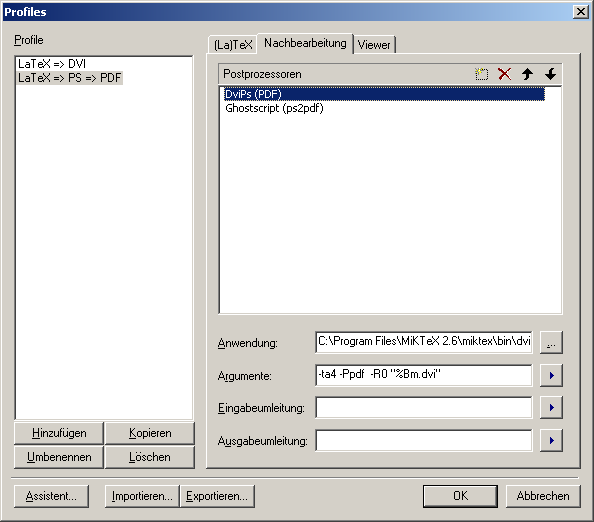
\includegraphics[width=0.49\textwidth]{techniccenter-profile-dvips-26} \\[4pt]
(a) & (b)
\end{tabular}
\caption{Spezifikation der Ausgabeprofile in TeXnicCenter.}
\label{fig:techniccenter-profile-latex}
\end{figure}

In der Datei \verb!tc_output_profiles_sumatra.tco! sind  folgende beiden "`maßgeschneiderten"' Ausgabeprofile für TexNicCenter angelegt (Import über \textsf{Build} $\rightarrow$ \textsf{Define Output Profiles ...}):
\begin{itemize}
	\item \verb!LaTeX => PDF (Sumatra)! -- Standard, direkte Erzeugung von PDF,
	\item \verb!LaTeX => PS => PDF (Sumatra)! -- PDF "`klassisch"' via DVI und PS.
\end{itemize}

\subsubsection{Profil "`\texttt{LaTeX => PDF (Sumatra)}"'}

Das ist das mit diesem Setup normalerweise verwendete Standardprofil.

\paragraph{(La)Tex:}
\begin{itemize}
  \item Path to the (La)TeX compiler: \\
        \begin{small} \verb!C:\Program Files (x86)\MiKTeX 2.9\miktex\bin\pdflatex.exe!\end{small}
  \item Command line arguments to pass to the compiler:\\
\begin{small}
   \verb!-synctex=-1 -interaction=nonstopmode "%pm"!
\end{small}
\end{itemize}

\paragraph{Postprocessor:} 
leer, kein Postprocessor notwendig.

\paragraph{Viewer:}
\begin{itemize}
\item Path of executable: \\
\begin{small}
    \verb!C:\Program Files (x86)\SumatraPDF\SumatraPDF.exe ! \\ 
    \verb!-inverse-search "\"C:\Program Files\TeXnicCenter\TEXCNTR.EXE\" !\\
    \verb!/ddecmd \"[goto('%f','%l')]\""!
\end{small}
%
\item View project's output: \\
\begin{small}
    \checkbox\ Command line argument \\\
    Command: \verb!"%bm.pdf"!
\end{small}
%
\item Forward search:\\
\begin{small}
    \checkbox\ DDE command \\\
    Command: \verb![ForwardSearch("%bm.pdf","%Wc",%l,0)]! \\
    Server: \verb!SUMATRA! \\
    Topic: \verb!Control!
\end{small}
\item Close document before running (La)TeX:\\
\begin{small}
    \checkbox\ Do not close
\end{small}
\end{itemize}


\subsubsection{Profil "`\texttt{LaTeX => PS => PDF (Sumatra)}"'}

Profil ausschließlich für den DVI-PS-Workflow (über DVI und PostScript).

\paragraph{(La)Tex:}
\begin{itemize}
  \item Path to the (La)TeX compiler: \\
        \begin{small} \verb!C:\Program Files (x86)\MiKTeX 2.9\miktex\bin\latex.exe!\end{small}
  \item Command line arguments to pass to the compiler:\\
\begin{small}
   \verb!-synctex=-1 -interaction=nonstopmode "%pm"!
\end{small}
\end{itemize}

\paragraph{Postprocessor:}
\begin{itemize}
  \item DviPS (PDF): \\
        \begin{small} 
        Executable: \verb!C:\Program Files (x86)\MiKTeX 2.9\miktex\bin\dvips.exe! \\
        Arguments: \verb!-ta4 -P pdf -R0 "%Bm.dvi"!
        \end{small}
  \item Ghostscript (ps2pdf):\\
  		\begin{small} 
        Executable: \verb!C:\Program Files (x86)\gs\gs9.04\bin\gswin32c.exe! \\
        Arguments: \verb!-q -dPDFSETTINGS=/prepress -sPAPERSIZE=a4 -dSAFER! \\
         \verb!-dBATCH -dNOPAUSE -sDEVICE=pdfwrite -sOutputFile="%bm.pdf"! \\
         \verb!-c save pop -f "%bm.ps"!
      \end{small}
\end{itemize}

\paragraph{Viewer:}
wie in Profil A. (\texttt{LaTeX => PDF (Sumatra)}).

\section{Tipps und offene Probleme:}

\begin{itemize}
\item \texttt{psfrag} funktioniert nicht mit \texttt{pdflatex} und es gibt auch leider keine Ersatzlösung. 
Wenn man \texttt{psfrag} braucht, dann muss man weiterhin über PostScript 
(\verb!LaTeX => PS => PDF!) arbeiten (was allerdings nunmehr auch mit \texttt{hyperref} kein Problem mehr ist).
%
\item Bei Verwendung des TexWorks-Editors (wird mit MikTeX ausgeliefert) sollte man die Standard-Zeichenkodierung von \emph{Unicode} (utf8) auf \emph{Latin-1} (ISO 8859-1) umstellen.
%
\item Adobe Illustrator kann beim Speichern als PDF die Bounding Box nicht setzen. 
Eine Möglichkeit ist, die Grafik zuerst als EPS zu exportieren und dann mit Acrobat in ein PDF zu konvertieren. 
%
\end{itemize}
\end{comment}



\begin{comment}
\section{Einstellungen für YAP (DVI-Viewer) im DVI-PS-Workflow}
\label{sec:YapEinstellung}

Im Standard-DVI-Viewer YAP lässt sich durch Mausklick auf das DVI-Dokument sehr leicht die zugehörige Stelle im Quelltext finden. Im Normalfall öffnet dann TeXnicCenter das zugehörige \latex-Dokument automatisch an der richtigen Stelle.
Das zugehörige "`Inverse DVI Search"' Kommando sollte sich bereits bei der Installation richtig einstellen.

Falls dies \emph{nicht} funktioniert, kann man in YAP diese Einstellung auch manuell über das Menü \textsf{View}\thinspace$\rightarrow$\thinspace\textsf{Options...} vornehmen, wie in Abb.\ \ref{fig:yap-inverse-search} gezeigt.
In diesem Fall lautet die vollständige Anweisung in "`Command Line"' folgendermaßen:
\begin{center}\footnotesize
\verb!"C:\Program Files (x86)\TeXnicCenter\TEXCNTR.EXE" /ddecmd "[goto('%f', '%l')]"!
\end{center}


\begin{figure}
\centering\small
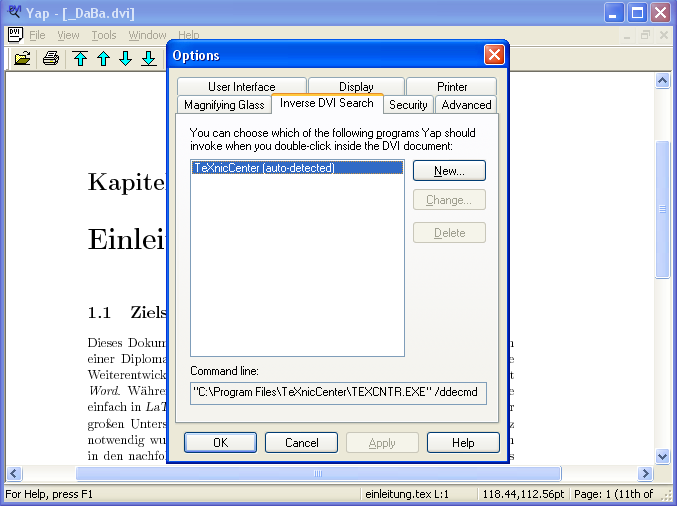
\includegraphics[width=1.0\textwidth]{yap-inverse-search-settings}
\caption{"`Inverse DVI Search"' Einstellung in YAP (über das Menü \textsf{View}\thinspace$\rightarrow$\thinspace\textsf{Options...}).}
\label{fig:yap-inverse-search}
\end{figure}

Latex
C:\Program Files\MiKTeX 2.6\miktex\bin\latex.exe
--src -interaction=nonstopmode "%Wm"

Bibtex
C:\Program Files\MiKTeX 2.6\miktex\bin\bibtex.exe
"%bm"

---

DviPs (PDF)
C:\Program Files\MiKTeX 2.6\miktex\bin\dvips.exe
-ta4 -Ppdf  -R0 "%Bm.dvi"

Ghostscript (ps2pdf)
C:\Program Files\gs\gs8.61\bin\gswin32c.exe
-sPAPERSIZE=a4 -dSAFER -dBATCH -dNOPAUSE -sDEVICE=pdfwrite -dPDFSETTINGS=/prepress -sOutputFile="%bm.pdf" -c save pop -f "%bm.ps"


YAP 
Options -> Inverse Search
"C:\Program Files\TeXnicCenter\TEXCNTR.EXE" /ddecmd "[goto('%f', '%l')]"

\end{comment}

	% Technische Ergänzungen
%\chapter{Contents of the CD-ROM}
\label{app:cdrom}

\paragraph{Format:}
		CD-ROM, Single Layer, ISO9660-Format%


\section{PDF files}
\begin{FileList}{/}
%\fitem{_DaBa.dvi} Gesamtdokument (DVI-File, ohne Grafiken)
\fitem{S1510629021_Zarhuber_Thesis.pdf} Master's Thesis with instructions (entire document)%
\end{FileList}

\begin{FileList}{/online}
  \fitem{Hexo 3.2.0-beta.2.pdf} \cite{Chen2015hexorelease}
  \fitem{Hexo debut.pdf} \cite{Chen2012hexodebut}
  \fitem{Hexo Documentation - Setup.pdf} \cite{HexoDocumentationSetup}
  \fitem{JSLint Documentation.pdf} \cite{JSLintDocumentation}
  \fitem{Node.js Documentation.pdf} \cite{NodejsChildProcesses}\cite{NodejsKillProcess}
  \fitem{Overview of Blocking vs Non-Blocking.pdf} \cite{NodejsBlockingNonblocking}
  \fitem{git-diff.pdf} \cite{GitDiff}
  \fitem{git-revert.pdf} \cite{GitRevert}
  \fitem{Introducing Markdown.pdf} \cite{Markdown2004introduction}
  \fitem{Markdown.pdf} \cite{Markdown2004main}
  \fitem{OAuth2orize.pdf} \cite{OAuth2orizeGitHub}
  \fitem{Routing.pdf} \cite{ExpressRouter}
  \fitem{Using middleware.pdf} \cite{ExpressMiddleware}
  \fitem{About pull requests.pdf} \cite{GithubPullRequests}
  \fitem{Basics of Authentication.pdf} \cite{GithubAuthentication}
  \fitem{Mastering Markdown.pdf} \cite{GithubFlavoredMarkdown}
  \fitem{Merging a pull request.pdf} \cite{GithubMergePullRequests}
  \fitem{Resolving a merge conflict using the command line.pdf} \cite{GitConflicts}
  \fitem{Webhooks.pdf} \cite{GithubWebhooks}
  \fitem{Write Scripts for the mongo Shell.pdf} \cite{MongoDBWritingScripts}
  \fitem{Building Technical Documentation with Metalsmith.pdf} \cite{Metalsmith2015technicaldocumentation}
  \fitem{Node based static site generators.pdf} \cite{Mann2012nodestaticsite}
  \fitem{JavaScript reference - Arrow functions.pdf} \cite{MDNArrowFunctions}
  \fitem{Using promises.pdf} \cite{MDNPromise}
  \fitem{Git Projects.pdf} \cite{PancakeGitProjects}
  \fitem{Blogging Like a Hacker.pdf} \cite{PrestonWerner2008jekyll}
  \fitem{GitHub Pages.pdf} \cite{PrestonWerner2008githubpages}
  \fitem{How I Turned Down USD 300,000.pdf} \cite{PrestonWerner2008githublaunch}
  \fitem{Directory structure.pdf} \cite{JekyllDirectoryStructure}
  \fitem{Usage of server-side programming languages for websites.pdf} \cite{W3TechLanguageTrends}
  \fitem{Setting up a Node.js Cluster.pdf} \cite{RobinsonNodeCluster}
  \fitem{Metalsmith Repository.pdf} \cite{MetalsmithRepository}
  \fitem{Building Building Blocks} \cite{Metalsmith2015buildingblocks}
\end{FileList}

\begin{FileList}{/source}
  \fitem{Technical Documentation.pdf} \latex version of the project's README.md
\end{FileList}


\section{Source code}
\begin{FileList}{/source}
  \fitem{v1.0.1.zip} Source code of the project
\end{FileList}


\section{Graphics}
\begin{FileList}{/images}
  \fitem{*.sketch} Source files
  \fitem{*.svg} Vector graphics
  \fitem{*.png} Rendered images \& Screenshots
\end{FileList}
	% Inhalt der CD-ROM/DVD
%\chapter{Chronologische Liste der Änderungen}


\begin{sloppypar}
\begin{description}
%
\item[2002/01/07]
\verb!\newfloat{program}! repariert (auch ohne Chapter). Dank an Werner Bailer!
%
\item[2002/03/06]
Copyright-Notice an internat.\ Standard angepasst. Dank an Karin Kosina!
%
\item[2002/07/28]
"`Studiengang"' $\rightarrow$ "`Diplomstudiengang"'
%
\item[2003/08/24]
Neues Macro: \verb!\Messbox{breite}{hoehe}! -- zur Kontrolle der 
Druckgröße ohne PS-Datei. Erweiterungen für Bakkalaureatsarbeiten
%
\item[2005/04/09]
Diverse Korrekturen: Captions von Tabellen nach oben gesetzt. 
\texttt{caption} auf neue Versionen adaptiert.
\texttt{subfigure} wird nicht mehr verwendet
%
\item[2006/01/20]
Adaptiert zur Verwendung als Praktikumsbericht 
(2.\ Bakk.-Arbeit)
%
\item[2006/03/24]
Fehler in \verb!\erklaerung! beseitigt (Dank an David Schwingenschlögl)
%
\item[2006/04/06]
Verwendung von T1-Fontencoding zur besseren Silbentrennung bei 
Umlauten etc.
%
\item[2006/06/21]
Neu: Bachelorstudiengang / Masterstudiengang.
Literaturverweise auf Bakk-Arbeiten.
\texttt{upquote.sty} eliminiert (Problem mit TS1-Kodierung).
Verwende Komma (statt Punkt) als Trennzeichen in Dezimalzahlen.
%
\item[2006/09/14]
Anmerkungen zum Thema Plagiarismus.
%
\item[2007/07/16]
Ergänzungen für Code-Listings (listings) und Algorithmen 
(\texttt{algorithmicx}).
BiBTeX-Datei aufgeräumt, Verwendung der Literaturformate 
verbessert.
Komma (statt Punkt) als Trennzeichen in Dezimalzahlen wieder 
entfernt.
Verwendung der \texttt{ae}-Fonts eliminiert (\texttt{cm-super} Fonts müssen 
installiert sein, ab MikTeX 2.5). 
Beispiel für Ersetzung in EPS-Dateien mit \texttt{psfrag}.
%
\item[2007/10/04]
Version 5.90: Das Laden der Pakete \verb!inputenc! (Option \texttt{latin}) und 
\verb!graphicx! (Option \texttt{dvips})
aus der Hauptdatei in die \texttt{sty}-Datei übertragen; \texttt{upquote} funktioniert nun.
Paket \texttt{eurosym} ergänzt für Euro-Symbol (Anregung von Andreas 
Doubrava).
Problem mit \texttt{color}-package repariert (gerasterter PDF-Ausdruck).
Hinweise bzgl.\ Literatur ergänzt (\texttt{month}, \texttt{edition}),
BibTeX-Datei gesäubert.
Hinweis zum Einfügen von vertikalem Abstand zwischen Absätzen.
Mathematik aufgeräumt, Verwendung von \texttt{amsmath}, 
Fallunterscheidungen.
Diverse Änderungen bei Tabellen und Programmkode.
Beispiele für BibTeX-Angaben von Spezialquellen: Audio-CDs, 
Videos, Filme. Einbinden von Dateien mit \verb!\include{..}!
Neue Datei: \verb!_SimpleReport.tex! für kurze Reports (Projekte etc.).
%
\item[2007/11/11]
Version 5.91: Hinweise zur Einstellung der Output-Profile in
TexNicCenter, Inverse Search Einstellung in YAP im Anhang.
%
\item[2008/04/01]
Version 6.00beta -- kompletter Umbau!
Auslagerung der Doku\-menten-relevanten Teile in eine eigene 
\emph{class}-Datei (\texttt{hgbthesis.cls}) mit Optionen.
Die neue Style-Datei \texttt{hgb.sty} ist nun unabhängig vom 
Dokumententyp und nicht mehr kompatibel mit älteren Versionen!
Die Liste der Änderungen ist jetzt in der Datei \verb!_ChangeLog.tex!
(DIESE Datei) und diese wird im Anhang eingebunden.
Heading-Style auf Sans Serif geändert (ohne grausliche "`Caps"').
%
\item[2008/05/22]
Neue Vorlage für Technical Reports (Klasse \texttt{hgbreport.cls}).
Spracheinstellung nunmehr mit \texttt{babel}-Paket, Hauptsprache
des Dokuments kann als Option der Klasse angegeben werden.
Sprachumschaltung innerhalb des Dokuments funktioniert nun
richtig. Mit der Sprachoption \texttt{german} wird automatisch die neue deutsche 
Orthographie (\texttt{ngerman}) verwendet.
\texttt{babelbib} wird zur Formatierung des Literaturverzeichnisses
verwendet (neue BibTeX-Style-Optionen!).
Header werden nunmehr mit \texttt{fancyhdr}-Paket erzeugt.
Versionsnummerierung von \texttt{.cls} und \texttt{.sty} Files wird beendet 
(ab jetzt gilt: \emph{Datum} = \emph{Version}). 
%
\item[2008/06/10]
Neues Listing-Environment \texttt{PhpCode}; bei allen Listing-Eviron\-ments ist nun 
\texttt{mathescape=false} (kein Math-Mode nach \verb!$!). 
Bug bei Sprachumschaltung auf \texttt{ngerman} beseitigt.
%
\item[2008/08/15]
Diverse Kleinigkeiten in Literaturangaben überarbeitet (Dank an Norbert Wenzel), Spracheinstellung vereinheitlicht, Umlaute in \texttt{.bib}-Datei ersetzt.
%
\item[2008/10/15] 
Zusätzliche Hinweise zur MikTeX-Installation (Windows) sowie LaTeX unter Mac OS~X und Linux.
Liste der Abkürzungen ergänzt.%
\item[2008/11/15] 
Diverse Schreibfehler korrigiert (Dank an Silvia Fuchshuber). Hinweis auf 
\texttt{sloppypar}-Umgebung.
%
\item[2008/12/09] 
BibTeX-Tools: neuer Hinweis auf JabRef ergänzt, BibEdit entfernt (ist nicht mehr auffindbar).
%
\item[2009/02/09]
\texttt{hgb.sty}: Option "`\texttt{spaces}"' zu \texttt{url}-Package ergänzt (ermöglicht gezielten Zeilenumbruch in URLs). 
Im allgemeinen Setup für \texttt{listings}: \texttt{keepspaces=true};
Obsoletes Environment \texttt{sourcecode} deaktiviert.
Escape-Mode für \texttt{LaTeXCode}-Umgebung geändert.
\verb!_DaBa.tex!: Hinweis auf die Verwendung von \verb!\urldef! für die Angabe von URLs in Captions. \texttt{diplom} (statt \texttt{master}) als Standard-Dokumententyp in \verb!_DaBa.tex! ("`Diplomarbeit"'). Neuer Abschnitt zum Umgang mit ``Quellenangaben in Captions''.
\texttt{literatur.bib}: alle URLs (bisher in \texttt{note}-Einträgen) auf \verb!url={..}! geändert.
%
\item[2009/04/14]
Hinweis zum Einfügen einfacher Anführungszeichen ergänzt.
%
\item[2009/07/18]
Literaturangaben korrigiert und ergänzt.
%
\item[2009/11/27]
Experimentelle Version: Massive Änderungen, Umstieg auf \texttt{pdflatex}.
%
\item[2010/06/15]
Erstes Release der neuen Version mit \texttt{pdflatex}.
\item[2010/06/23]
Konflikt zwischen \texttt{pdfsync}-Package und \texttt{array}-Package (wird relativ häufig benutzt) durch \verb!\RequirePackage[novbox]{pdfsync}! behoben.
Seitenunterkante durch \verb!\flushbottom! fixiert,
variablen Absatzzwischenraum reduziert.
\item[2010/07/27]
Sprache der Erklärungsseite auf "`\texttt{german}"' fixiert (auch wenn die Hauptsprache des Dokuments  Englisch ist). %Datumsproblem - Hinweis von Philipp Winter
\item[2010/12/03]
Anmerkungen und Beispiele zum Zitieren von Gesetzestexten und Videos (Zeitangabe) ergänzt.
Hinweis auf \verb!\nolinkurl{..}! zur Angabe von Dateinamen.
\item[2011/01/29]
Einbau der Creative Commons Lizenz und entsprechender Hinweis in 
Abschnitt \ref{sec:HagenbergEinstellungen}. Neue Makros
\verb!\strictlicense!,
\verb!\cclicense! und
\verb!\license{...}!.
BibTeX-Einträge für Audio-CDs und Filme korrigiert, Beispiel für Online-Video ergänzt.
\item[2011/02/01]
Neues Makro \verb!\betreuerin{..}! zur Angabe einer (weiblichen) Betreuerin. 
%
\item[2011/06/26]
Umstellung der gesamten Literaturverwaltung auf \texttt{biblatex} mit dem Ziel, 
getrennte Abschnitte für verschiedene Kategorien von Einträgen im Quellenverzeichnis
zu ermöglichen. Die Wahl fiel auf \texttt{biblatex} (es gäbe andere Optionen), weil
damit BibTeX weiterhin nur einmal aufgerufen werden muss (und nicht für
mehrere Dateien). Damit verbunden sind allerdings massive Änderungen bei der
Syntax der BibTeX-Felder und es gibt auch mehrere neue Felder.
Aktuell sind 3 Kategorien von Quellen vorgesehen, entsprechende Änderungen in 
\nolinkurl{hgbthesis.cls}. Der klassische BibTeX-Workflow wird aktuell nicht
mehr unterstützt, die Möglichkeit einer künftigen Dok-Option ist aber 
vorgesehen. Das Literatur-Kapitel ist komplett überarbeitet, die .bib-Datei
wurde ausgemistet. Neu ist die Empfehlung zur Aufnahme von Bildquellen
in das Quellenverzeichnis, womit lange URLs in Captions (dort sind keine
Fußnoten möglich) nicht mehr notwendig sind. 
"`Persönliche Kommunikation"' als Literaturquelle entfernt (den Inhalt
von Interviews sollte man direkt im Anhang wiedergeben).
Das verwendete Bildmaterial wurde
erneuert, aktuell werden nur mehr Public Domain Bilder verwendet. 
Das Kapitel "`Hinweise für Word-Benutzer"' wurde endgültig entfernt.
\verb!\flushbottom! wieder auf \verb!\raggedbottom! geändert, um übermäßige 
Abstände zwischen Absätzen zu vermeiden.
%
\item[2012/05/10]
Hinweis auf die in Österreich bislang nicht zulässige Verwendung von "`Masterarbeit"'
entfernt, \texttt{master} ist nunmehr die Default-Dokumentenoption.
Anmerkungen zu lästigen \texttt{biblatex}-Warnungen ergänzt.
Angaben für Windows-Programmpfade auf Win7 angepasst, 
MikTeX 2.9 als Minimalerfordernis.\newline
Überflüssige Makros \verb!\damonat! und \verb!\dajahr! endgültig entfernt, statt
\verb!\abgabemonat! und \verb!\abgabejahr! ist nun das neue Makro
\verb!\abgabedatum{yyyy}{mm}{dd}! vorgesehen (unter Verwendung von internen Zählern).
Zur Formatierung von Datumsangaben wir das \texttt{datetime}-Paket verwendet.
\newline
Neue Fassung der eidesstattlichen Erklärung (inkl.\ englischer Version).\newline
PDF-Suche auf \texttt{synctex} umgestellt (\texttt{pdfsync}-Paket ist veraltet und
wird nun nicht mehr verwendet).
\newline
Die älteren Dateiversionen von \texttt{algorithmicx.sty} und \texttt{alg\-pseudo\-code.sty}
(bisher explizit beigefügt) wurden weggelassen.
\newline
Hinweis auf die \emph{Latin Modern Roman} OTF-Schriften ergänzt.
%
\item[2012/07/21]
Quellenverzeichnis: sprachabhängige Einstellung der Überschriften eingerichtet.
Titel des Quellenverzeichnisses auf "`Quellenverzeichnis"' (DE) \bzw\ "`References"' (EN) 
fixiert. Makro \verb!\MakeBibliography! hat damit keinen erforderlichen Parameter mehr.
%
\item[2012/09/17]
Wegen Änderungen im \texttt{biblatex}-package (Version 1.7, 2011/11/13) die Verwendung von
BibTeX als backend eingestellt (\texttt{backend=bibtex8}).
%
\item[2012/10/13]
Option \texttt{lowtilde} beim URL-package eingestellt (erzeugt \url{~} statt \verb!~!).
%
\item[2012/12/01]
In Abschnitt \ref{sec:FormatierungVonProgrammcode} zusätzliche Code-Umgebungen ergänzt:
\texttt{JsCode},
\texttt{PhpCode},
\texttt{HtmlCode},
\texttt{CssCode},
\texttt{XmlCode}.
%
\item[2012/12/08]
Die Code-Umgebungen in Abschn.\ \ref{sec:FormatierungVonProgrammcode} ergänzt und 
zur Verwendung von optionalen Argumenten erweitert (Hinweise in Abschnitt 
\ref{sec:FormatierungVonProgrammcode} auf die Argumente
\texttt{firstnumber=last} und \texttt{numbers=none}).
Quellenverzeichnis: den Eintragstyp \texttt{@software} für Games empfohlen und im Verzeichnis
der Kategorie \emph{avmedia} zugeordnet (Tab.~\ref{tab:BibKategorien} ergänzt). 
Game-Beispiel (von Manuel Wieser) und zusätzliche Tabelle \ref{tab:QuellenUndEintragstypen}
zur besseren Übersicht eingefügt.
%
\item[2013/05/17]
Wichtigste Änderung ist die vollständige Umstellung auf \textbf{UTF-8} unter Beibehaltung des 
\texttt{pdflatex}-Workflows. 
Damit sind zahlreiche weitere Modifikationen verbunden:
\newline
Alle Dateien (auch \texttt{.cls}, \texttt{.sty} und \texttt{.bib}) wurden auf UTF-8 konvertiert.
Damit sollte es auch keine Probleme mehr mit Umlauten und Sonderzeichen unter MacOS geben.
\newline
Die verwendete Standard-Schriftfamilie ist nun "`Latin Modern"' (\texttt{lmodern}). 
Sie ersetzt die "`CM-Super"' Schriften, mit denen es immer wieder Installationsprobleme gab.
Weiters wird jetzt das \texttt{cmap}-Paket zur besseren Such- und Kopierbarkeit von PDFs verwendet.
\newline
Das \texttt{listings}-Paket wurde durch \texttt{listingsutf8} ersetzt und für Umlaute im Quellcode adaptiert.
Eventuell sind weitere Adaptierungen notwendig.
\newline
\texttt{biber} (min.\ Version 1.5!) wird nun anstatt \texttt{bibtex} (unterstützt keine UTF-8 Dateien) verwendet,
zusammen mit \texttt{biblatex} (Version 2.5).
Die Anweisung \verb!\bibliography! wird (wieder) verwendet, allerdings nun in der Präambel,
um die \texttt{.bib}-Datei im Fileverzeichnis anzuzeigen.
\newline
Das Makro \verb!\C! (für die Menge der komplexen Zahlen \Cpx) musste wegen Problemen in der T1-Kodierung
ersetzt werden und heißt nun \verb!\Cpx!. Die Makros 
\verb!\R!, \verb!\Z!, \verb!\N!, \verb!\Q! und \verb!\Cpx! können nun auch außerhalb des Mathematik-Modus verwendet werden.
\newline
Der DVI-PS-PDF Workflow wird ab dieser Version überhaupt nicht mehr unterstützt. 
Damit ist auch das \texttt{psfrag}-Paket nicht mehr verwendbar. Entspechende Hinweise 
wurden aus dem Text entfernt.
\newline
\texttt{hyperref} wurde auf UTF-8 umgestellt.
Die grässlichen Standard-Rahmen und Farben der automatischen \texttt{hyperref}-Links wurden entfernt \bzw\ durch 
dezentere Farben ersetzt. Dadurch wird auch die Screen-Version der PDFs wieder lesbar.
\newline
Im Quellenverzeichnis wurde versuchsweise die \texttt{backref}-Option aktiviert. 
Damit werden bei allen Einträgen auch die zugehörigen Zitierstellen angegeben
(erscheint durchaus sinnvoll).
\newline
Die bisherigen Korrekturen zur \texttt{biblatex}-Formatierung wurden entfernt, 
alles arbeitet nun mit Standard-Einstellungen. Die ursächlichen Probleme in \texttt{biblatex}
scheinen in der aktuellen Version behoben zu sein.
\newline
Das Output-Profil für TeXnicCenter wurde für den neuen Workflow mit \texttt{biber} adaptiert und liegt nun in
\nolinkurl{_tc_output_profile_sumatra_utf8.tco}.
\newline
Das Windows-Script \verb!_clean.bat! wurde entfernt, da TeXnicCenter nun ein eigenes "`Clean Project"'-Kommando aufweist (in "`Build"').
\newline
Allgemeine Einstellungen zu \emph{headings} und \emph{biblatex} wurden aus der Datei \texttt{hgbthesis.cls} entfernt und in 
\texttt{hgbheadings.sty} \bzw\ \texttt{hgbbib.sty} verlagert. Diese können nun unabhängig verwendet werden (s.\ Beispiel in 
\texttt{\_TermReport.tex}).
\newline
Die Klassen-Datei \texttt{hgbtermreport.cls} wurde eliminiert, das Dokument \texttt{\_TermReport.tex} basiert nunmehr
auf der generischen LaTeX-Klasse \texttt{report}  und verwendet keine eigene \texttt{.cls} Datei mehr.
%
\item[2014/11/05]
Neu: Logo auf der Frontseite bei allen Dokumententypen. Dazu gibt es ein neues Kommando
\verb!\logofile{pic}!, wobei \verb!pic! der Name eine PDF-Datei im
Verzeichnis \verb!images/! ist. Falls \emph{kein} Logo erwünscht ist, 
kann man die Zeile einfach weglassen oder durch \verb!\logofile{}! ersetzen.
\newline
\texttt{hyperref}-Einstellungen: Einfärbung der Links wieder entfernt (\texttt{colorlinks = false}), weil beim Druck
nicht abschaltbar. Stattdessen einheitliche (dezente) Rahmen für alle Linkarten.
Zahlreiche Tippfehler eliminiert (Dank an Daniel Karzel).
\newline
Wegen eines Bugs in \texttt{biblatex 1.9} wurden die expliziten Abteilungen (\verb!\-!) in \texttt{literatur.bib}
vorübergehend entfernt (mit entsprechenden Folgen im Ergebnis). Der Bug soll in \texttt{biblatex 2.0} (derzeit noch
nicht verfügbar) behoben sein.
\newline
Package \texttt{color} auf \texttt{xcolor} geändert. In \texttt{hgb.sty} neues "`Convenience-Makro"' \verb!\etc! ergänzt.
Output-Profil für TeXnicCenter/SumatraPDF (Windows) repariert, forward/inverse Search funktioniert nun
(Datei \verb!_tc_output_profile_sumatra_utf8.tco!).
%
\item[2015/04/28]
Paket \texttt{subdepth} (zur verbesserten Platzierung von Sub- und Superscripts) 
in hgb.sty ergänzt.
%
\item[2015/07/14]
Hinweis und Abhilfe für die (nicht automatische) Silbentrennung in zusammengesetzten Wörtern.
Neu in \texttt{hgbheadings.sty}: \verb!\RequirePackage[raggedright]{titlesec}! verhindert Blocksatz
in Section-Überschriften (sehr unschön bei längeren Überschriften). 
Neu (in Abschn.~\ref{sec:GraphicOverlays}): Beispiel für die Verwendung des \texttt{overpic}-Pakets
zur Annotierung von importierten Grafiken (verwendet zudem das \texttt{pict2e}-Paket).
%
\item[2015/08/03]
Logo-Datei auf \texttt{logo.pdf} umbenannt.
\item[2015/09/17]
Anweisung \verb!\RequirePackage[utf8]{inputenc}! in die Doku\-menten\-dateien (\texttt{\_xxx.tex})
verschoben (auf Anregung von Markus Kohm: "`\ldots für die Verwendung von lualatex oder xelatex 
ist die Anweisung in hgb.sty störend, da bei diesen beiden aufgrund der nativen utf8-Unterstützung 
\texttt{inputenc} keinesfalls verwendet werden darf"').
\item[2015/09/19]
\texttt{hgb.sty} aufgeräumt.
Makros \verb!\@savesymbol! und \verb!\@restoresymbol! aus \texttt{hgb.sty} entfernt
(wurden nicht mehr verwendet; ggfs.\ Paket \texttt{savesym} als Ersatz).
Makro \verb!\optbreaknh! (optional break with no hyphen) auf \verb!\obnh! umbenannt.
Teile von \texttt{hgb.sty} in neue Dateien \texttt{hgbabbrev.sty} (div.\ Abkürzungen)
und \texttt{hgblistings.sty} (Code-Listings) verschoben.
Hintergrundtönung der Code-Listings heller (auf 5\% Grau) eingestellt.
Layout: \verb!\textfraction! auf 0.1 (statt fehlhafterweise 0.01) eingestellt.
\texttt{hgbbib.sty}: \verb!\clearpage! am Beginn des Quellenverzeichnisses entfernt
(für \texttt{article}-Template).
\item[2015/09/19]
Alle \texttt{.cls} und \texttt{.sty} Dateien sind jetzt ANSI-codiert (Header eingefügt), wie
laut CTAN-Richtlinien vorgesehen. Umlautzeichen wurden durch Makros ersetzt.
Nur \texttt{hgblistings.sty} ist weiterhin UTF-8 (wegen notwendiger literaler Umlaute).
\verb!\RequirePackage[utf8]{inputenc}! steht sonst nur mehr am Beginn
der jeweiligen (\texttt{.tex}) Haupttextdatei.
\item[2015/10/29]
Verwendung von "`In:"' im Quellenverzeichnis vor \texttt{article}-Einträgen
(Eigenart von biblatex) durch passendes Makro in \texttt{hgbbib.sty} unterbunden 
(Dank an S.\ Dreiseitl).
\item[2015/11/04]
Hinweise in Abschnitt \ref{sec:Software} auf TeXstudio unter Windows, Mac OS und Linux.
Release-Ausgabe.
\item[2015/12/08]
Source Directories neu strukturiert in \texttt{frontmatter}, \texttt{chapters}, 
\texttt{appendix}.
\item[2016/06/09]
Bibliography-Aliases für die Quellentypen
\texttt{video}, \texttt{movie}, \texttt{audio} und \texttt{software}
eingefügt (in \texttt{hgbbib.sty}) -- unterbindet Warnungen wegen
fehlender biblatex-Driver.
\item[2016/06/11]
Repository portiert auf GitHub (SourceForge eingefroren).  
Overleaf als experimentelle online LaTeX-Umgebung.
Hauptdateien umbenannt (auf \texttt{\_thesis}, \texttt{\_praktikum}, etc.).
\end{description}
\end{sloppypar}




%\section*{To Do} 
%\begin{itemize}
%\item Inkscape
%\item biblatex Bib-Driver für audio, video etc. ergänzen.
%\item Mathematik umbauen, typische Fehler stärker berücksichtigen (ua. Leerzeilen vor/nach Gleichungen).
%\item Literaturempfehlungen zum Schreiben von Diplomarbeiten
%\item Hinweise für Literatursuche (Bibliotheksverbund, CiteSeer,...)
%\end{itemize}





	% Chronologische Liste der Änderungen
%\chapter{\latex-Quellkode}
\label{app:latex}

\section*{Hauptdatei {\tt\_DaBa.tex}}

\begin{footnotesize}
\verbatiminput{_DaBa.tex}
\end{footnotesize}


%\vspace*{2cm}
\hrule
\hrule

\paragraph{Anmerkung:}
Das sollte nur ein \emph{Beispiel} für die Einbindung von Quellcode
in einem Anhang sein. Der \latex-Quellkode der eigenen
Abschlussarbeit ist meist \emph{nicht} interessant genug, um ihn hier
wiederzugeben!

	% Quelltext dieses Dokuments

%%%----------------------------------------------------------
\MakeBibliography                        % Quellenverzeichnis
%%%----------------------------------------------------------

%%% Messbox zur Druckkontrolle ------------------------------
\chapter*{Messbox zur Druckkontrolle}



\begin{center}
{\Large --- Druckgröße kontrollieren! ---}

\bigskip

\Messbox{100}{50} % Angabe der Breite/Hoehe in mm

\bigskip

{\Large --- Diese Seite nach dem Druck entfernen! ---}

\end{center}



%%%----------------------------------------------------------
\end{document}
%%%----------------------------------------------------------
